% Titre : trigo
% Filiere : BCPST
% Difficulte : 
% Type : TD 
% Categories :trigo
% Subcategories : 
% Keywords : trigo




\begin{exercice}   \;
R\'esoudre les in\'equations suivantes dans $\R$, puis dans $\lbrack 0,2\pi\lbrack$ et $\rbrack -\pi,\pi\rbrack$ :
\begin{enumerate}
\begin{minipage}[t]{0.45\textwidth}
\item $2\sin{x}-1<0$
\item $2\cos{(2x)}>\sqrt{3}$
\item $\ddp\frac{1}{\sqrt{3}}\tan{(3x)}>1$
\end{minipage}
\begin{minipage}[t]{0.45\textwidth}
\item $\sin{(3x)}\geq -\ddp\frac{\sqrt{3}}{2}$
\item $\sqrt{2}\cos{(3x)}\leq 1$
\item $\tan{(x)}\leq 1$
\end{minipage}
\end{enumerate}
\end{exercice}


\%\%\%\%\%\%\%\%\%\%\%\%\%\%\%\%\%\%\%\%
\%\%\%\%\%\%\%\%\%\%\%\%\%\%\%\%\%\%\%\%
\%\%\%\%\%\%\%\%\%\%\%\%\%\%\%\%\%\%\%\%




\begin{correction}   \;
\begin{enumerate}
%------------------------------
\item \textbf{R\'esolution de $\mathbf{2\sin{(x)}-1<0}$:}  On se ram\`ene \`a une in\'equation fondamentale :$2\sin{x}-1<0  \Leftrightarrow \sin{x}<\ddp\frac{1}{2}.$\\
On r\'esout alors cette in\'equation fondamentale graphiquement:\\
\begin{minipage}[c]{0.45\textwidth}
\fbox{$ \mathcal{S}_{\R}= \ddp \mathop{\bigcup}\limits_{k\in \Z} \left] - \frac{7\pi}{6} + 2k\pi , \frac{\pi}{6} + 2k \pi \right[$}.\\
Et on a : \conclusion{$\mathcal{S}_{\lbrack 0,2\pi\lbrack}=\left\lbrack 0,\ddp\frac{\pi}{6}\right\lbrack\cup\left\rbrack \ddp\frac{5\pi}{6},2\pi\right\lbrack$}.\\
Et finalement : \conclusion{$ \mathcal{S}_{\rbrack -\pi,\pi\rbrack}=\left\rbrack -\pi,\ddp\frac{\pi}{6}\right\lbrack\cup\left\rbrack \ddp\frac{5\pi}{6},\pi\right\rbrack.$}
\end{minipage}
\quad 
\begin{center}
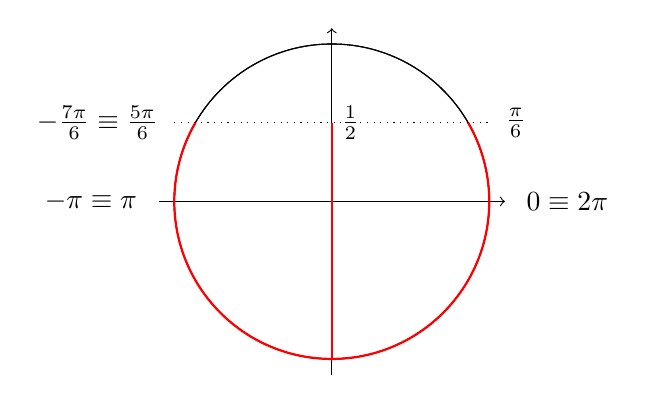
\begin{tikzpicture}[scale=2]
%Axes
\draw [->] (-1.1,0) -- (1.1,0);
\draw [->] (0,-1.1) -- (0,1.1);
%Cercle
\draw (0,0) circle (1);
%Intervalles axes
\draw [red,{-[}, thick] (0,-1) -- (0,0.5) ;
%Traits
\draw [dotted] (-1,0.5) -- (1,0.5) ;
%Points
\draw (0,0.5) node[right] {$\ddp \frac{1}{2}$};
\draw (1,0) arc (0:-210:1) node[left] {$\ddp - \frac{7\pi}{6} \equiv \frac{5\pi}{6} \quad $} ;
\draw (1,0) arc (0:30:1) node[right] {$\quad \ddp \frac{\pi}{6}$} ;
\draw (1,0) arc (0:0:1) node[right] {$\quad 0 \equiv 2\pi$} ;
\draw (1,0) arc (0:180:1) node[left] {$ -\pi \equiv \pi \quad$} ;
%Intervalles cercle
\draw [red, {-[}, thick] (1,0) arc (0:30:1) ;
\draw [red, {-[}, thick] (1,0) arc (0:-210:1) ;
\end{tikzpicture}
\end{center}

%------------------------------
\item \textbf{R\'esolution de $\mathbf{2\cos{(2x)}>\sqrt{3}}$:} On se ram\`ene \`a une in\'equation fondamentale :
$$2\cos{(2x)}>\sqrt{3}  \Leftrightarrow \cos{(2x)}>\ddp\frac{\sqrt{3}}{2}\quad (\star).$$
\begin{minipage}[c]{0.45\textwidth}
On r\'esout alors cette in\'equation fondamentale graphiquement:\\
$$\begin{array}{lll}
(\star) & \Leftrightarrow & \exists k\in\Z,\ -\ddp\frac{\pi}{6}+2k\pi <  2x < \ddp\frac{\pi}{6}+2k\pi\vsec\\
&\Leftrightarrow & \exists k\in\Z,\ -\ddp\frac{\pi}{12}+k\pi <  x < \ddp\frac{\pi}{12}+k\pi.
\end{array}$$
\end{minipage}
\quad \begin{minipage}[c]{0.45\textwidth}
\begin{center}
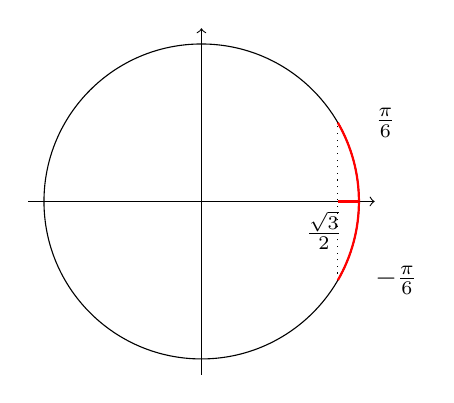
\begin{tikzpicture}[scale=2]
%Axes
\draw [->] (-1.1,0) -- (1.1,0);
\draw [->] (0,-1.1) -- (0,1.1);
%Cercle
\draw (0,0) circle (1);
%Intervalles axes
\draw [red,{]-}, thick] (0.866,0) -- (1,0) ;
%Traits
\draw [dotted] (0.866,-0.5) -- (0.866,0.5) ;
%Points
\draw (0.866,0) node[left, below] {$\ddp \frac{\sqrt{3}}{2} \quad$};
\draw (1,0) arc (0:-30:1) node[right] {$\quad \ddp - \frac{\pi}{6} $} ;
\draw (1,0) arc (0:30:1) node[right] {$\quad \ddp \frac{\pi}{6}$} ;
%Intervalles cercle
\draw [red, {-[}, thick] (1,0) arc (0:30:1) ;
\draw [red, {-[}, thick] (1,0) arc (0:-30:1) ;
\end{tikzpicture}
\end{center}
\end{minipage}
On obtient donc : $\fbox{$ \mathcal{S}_{\R}= \ddp \mathop{\bigcup}\limits_{k\in \Z} \left] - \frac{\pi}{12} + k\pi , \frac{\pi}{12} + k \pi \right[$}.$\\
Bien penser \`a refaire un deuxi\`eme cercle pour tracer les solutions, et pouvoir en d\'eduire les solutions sur les intervalles demand\'es. \\
\begin{minipage}[c]{0.45\textwidth}
On a :
$$\fbox{$\mathcal{S}_{\lbrack 0,2\pi\lbrack}=\left\lbrack 0,\ddp\frac{\pi}{12}\right\lbrack\cup\left\rbrack \ddp\frac{11\pi}{12},\ddp\frac{13\pi}{12}\right\lbrack\cup\left\rbrack \ddp\frac{23\pi}{12},2\pi\right\lbrack$}.$$
Et finalement :
 $$\fbox{$\mathcal{S}_{\rbrack -\pi,\pi\rbrack}=\left\rbrack -\pi,-\ddp\frac{11\pi}{12}\right\lbrack\cup\left\rbrack -\ddp\frac{\pi}{12},\ddp\frac{\pi}{12}\right\lbrack\cup\left\rbrack \ddp\frac{11\pi}{12},\pi\right\rbrack.$}$$
 \end{minipage}
\quad \begin{minipage}[c]{0.45\textwidth}
\begin{center}
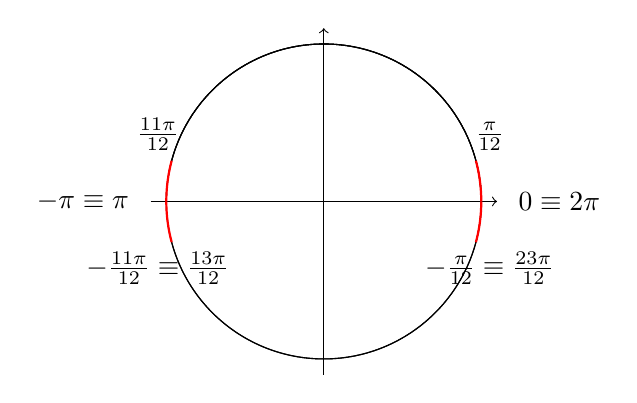
\begin{tikzpicture}[scale=2]
%Axes
\draw [->] (-1.1,0) -- (1.1,0);
\draw [->] (0,-1.1) -- (0,1.1);
%Cercle
\draw (0,0) circle (1);
%Points
\draw (1,0) arc (0:15:1) node[above] {$\quad \ddp \frac{\pi}{12}$} ;
\draw (1,0) arc (0:-15:1) node[below] {$\quad \ddp -\frac{\pi}{12} \equiv \frac{23\pi}{12}$} ;
\draw (1,0) arc (0:165:1) node[above] {$ \ddp \frac{11\pi}{12}\quad$} ;
\draw (1,0) arc (0:-165:1) node[below] {$\ddp -\frac{11\pi}{12} \equiv \frac{13\pi}{12}\quad$} ;
\draw (1,0) arc (0:0:1) node[right] {$\quad 0 \equiv 2\pi$} ;
\draw (1,0) arc (0:180:1) node[left] {$ -\pi \equiv \pi \quad$} ;
%Intervalles cercle
\draw [red, {-[}, thick] (1,0) arc (0:-15:1) ;
\draw [red, {-[}, thick] (1,0) arc (0:15:1) ;
\draw [red, {-[}, thick] (-1,0) arc (180:165:1) ;
\draw [red, {-[}, thick] (-1,0) arc (180:195:1) ;
\end{tikzpicture}
\end{center}
\end{minipage}
%-----------------------------
\item \textbf{R\'esolution de $\mathbf{\ddp\frac{1}{\sqrt{3}}\tan{(3x)>1 }}$:} On se ram\`ene \`a une in\'equation fondamentale :
$$\ddp\frac{1}{\sqrt{3}}\tan{(3x)}>1  \Leftrightarrow \tan{(3x)}>\sqrt{3}\quad (\star)$$
\begin{minipage}[c]{0.45\textwidth}
On r\'esout alors cette in\'equation fondamentale graphiquement:\\
$$\begin{array}{lll}
(\star)&\Leftrightarrow & \exists k\in\Z,\ \ddp\frac{\pi}{3}+k\pi <  3x < \ddp\frac{\pi}{2}+k\pi\vsec\\
&\Leftrightarrow & \exists k\in\Z,\ \ddp\frac{\pi}{9}+\ddp\frac{k\pi}{3} <  x < \ddp\frac{\pi}{6}+\ddp\frac{k\pi}{3}.
\end{array}$$
On obtient :
%$$\fbox{$ \mathcal{S}_{\R}=\left\lbrace x\in\R,\ \exists k\in\Z,\   \ddp\frac{\pi}{9}+\ddp\frac{k\pi}{3} <  x < \ddp\frac{\pi}{6}+\ddp\frac{k\pi}{3}\right\rbrace.$}$$
$$\fbox{$ \mathcal{S}_{\R}= \ddp \mathop{\bigcup}\limits_{k\in \Z} \left] \frac{\pi}{9} + \frac{k\pi}{3} , \frac{\pi}{6} + \frac{k \pi}{3} \right[$}.$$
\end{minipage}
\quad \begin{minipage}[c]{0.45\textwidth}
\begin{center}
\begin{tikzpicture}[scale=2]
%Axes
\draw [->] (-1.1,0) -- (1.1,0);
\draw [->] (0,-1.1) -- (0,1.1);
\draw (1,-1.1) -- (1,2);
%Cercle
\draw (0,0) circle (1);
%Intervalles axes
\draw [red,{]-}, thick] (1,1.732) -- (1,2);
%Traits
\draw [dotted] (0,0) -- (1,1.732) ;
%Points
\draw (1,1.732) node[right] {$\quad \ddp \sqrt{3}$};
\draw (1,0) arc (0:90:1) node[above] {$\quad \ddp \frac{\pi}{2} $} ;
\draw (1,0) arc (0:60:1) node[right] {$\quad \ddp \frac{\pi}{3}$} ;
%Intervalles cercle
\draw [red, {]-[}, thick] (0,1) arc (90:60:1) ;
\end{tikzpicture}
\end{center}
\end{minipage}
On refait alors un autre cercle trigonom\'etrique (\`{a} faire) afin de placer les angles solutions et on obtient, en prenant $k\in\intent{ 0,5}$ : \conclusion{$\mathcal{S}_{\lbrack 0,2\pi\lbrack}=\left\rbrack \ddp\frac{\pi}{9},\ddp\frac{\pi}{6} \right\lbrack\cup\left\rbrack \ddp\frac{4\pi}{9},\ddp\frac{\pi}{2} \right\lbrack\cup\left\rbrack \ddp\frac{7\pi}{9},\ddp\frac{5\pi}{6} \right\lbrack\cup\left\rbrack \ddp\frac{10\pi}{9},\ddp\frac{7\pi}{6} \right\lbrack\cup\left\rbrack \ddp\frac{13\pi}{9},\ddp\frac{3\pi}{2} \right\lbrack\cup\left\rbrack \ddp\frac{16\pi}{9},\ddp\frac{11\pi}{6} \right\lbrack .$}
Enfin, on a : \conclusion{$\ddp \mathcal{S}_{]-\pi,\pi]}=\left]-\frac{8\pi}{9}, -\frac{5\pi}{6} \right[ \cup \left] - \frac{5\pi}{9}, - \frac{\pi}{2}\right[ \cup \left] -\frac{\pi}{3}, -\frac{\pi}{6}\right[ \cup \left\rbrack \ddp\frac{\pi}{9},\ddp\frac{\pi}{6} \right\lbrack\cup \left\rbrack \ddp\frac{4\pi}{9},\ddp\frac{\pi}{2} \right\lbrack \cup \left\rbrack \ddp\frac{7\pi}{9},\ddp\frac{5\pi}{6} \right\lbrack$}.
%------------------------------
\item \textbf{R\'esolution de $\mathbf{ \sin{(3x)} \geq -\ddp\frac{\sqrt{3}}{2}}$:}\\
\begin{minipage}[c]{0.45\textwidth}
\noindent  La r\'esolution graphique sur le cercle trigonom\'etrique donne: 
$$\begin{array}{rcl}
\ddp \sin{(3x)}\geq -\ddp\frac{\sqrt{3}}{2} & \Leftrightarrow & \ddp \exists k\in\Z,\ -\ddp\frac{\pi}{3}+2k\pi\leq 3x\leq \ddp\frac{4\pi}{3}+2k\pi\vsec\\
&  \Leftrightarrow & \ddp \exists k\in\Z,\ -\ddp\frac{\pi}{9}+\frac{2k\pi}{3} \leq x \leq \ddp\frac{4\pi}{9}+\frac{2k\pi}{3}
\end{array} $$
On obtient donc : 
$$\fbox{$ \mathcal{S}_{\R}= \ddp \mathop{\bigcup}\limits_{k\in \Z} \left[ -\frac{\pi}{9} + \frac{2 k\pi}{3} , \frac{4\pi}{9} + \frac{2k \pi}{3} \right]$}.$$
\end{minipage}
%quad \begin{minipage}[c]{0.45\textwidth}
\begin{center}
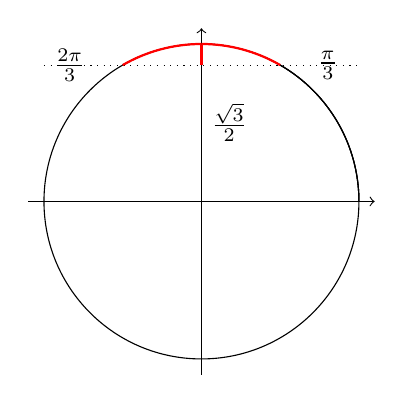
\begin{tikzpicture}[scale=2]
%Axes
\draw [->] (-1.1,0) -- (1.1,0);
\draw [->] (0,-1.1) -- (0,1.1);
%Cercle
\draw (0,0) circle (1);
%Intervalles axes
\draw [red,{[-}, thick] (0,0.866) -- (0,1) ;
%Traits
\draw [dotted] (-1,0.866) -- (1,0.866) ;
%Points
\draw (0,0.5) node[right] {$\ddp \frac{\sqrt{3}}{2}$};
\draw (1,0) arc (0:120:1) node[left] {$\ddp \frac{2\pi}{3} \quad $} ;
\draw (1,0) arc (0:60:1) node[right] {$\quad \ddp \frac{\pi}{3}$} ;
%Intervalles cercle
\draw [red, {-]}, thick] (0,1) arc (90:60:1) ;
\draw [red, {-]}, thick] (0,1) arc (90:120:1) ;
\end{tikzpicture}
\end{center}

On fait un cercle trigonom\'etrique pour placer les solutions, et on obtient, en prenant $k \in \intent{ 0, 2 }$ :
$$ \fbox{$\mathcal{S}_{\lbrack 0,2\pi\lbrack}=\left\lbrack 0,\ddp\frac{4\pi}{9} \right\rbrack\cup\left\lbrack \ddp\frac{5\pi}{9},\ddp\frac{10\pi}{9} \right\rbrack\cup\left\lbrack \ddp\frac{11\pi}{9},\ddp\frac{16\pi}{9} \right\rbrack\cup\left\lbrack \ddp\frac{17\pi}{9},2\pi \right\lbrack$}.$$
Et finalement :
$$ \fbox{$\mathcal{S}_{\rbrack -\pi,\pi\rbrack}=\left\rbrack -\pi,-\ddp\frac{8\pi}{9} \right\rbrack\cup\left\lbrack -\ddp\frac{7\pi}{9},-\ddp\frac{2\pi}{9} \right\rbrack\cup\left\lbrack -\ddp\frac{\pi}{9},\ddp\frac{4\pi}{9} \right\rbrack\cup\left\lbrack \ddp\frac{5\pi}{9},\pi \right\rbrack$}.$$
%------------------------------
\newpage
\item \textbf{R\'esolution de $\mathbf{ \sqrt{2}\cos{(3x)}\leq 1 }$:}\\
\noindent On a: $ \sqrt{2}\cos{(3x)}\leq 1 \Leftrightarrow \cos{(3x)}\leq \ddp\frac{1}{\sqrt{2}}$. \\
\begin{minipage}[c]{0.45\textwidth}
La r\'esolution sur le cercle trigonom\'etrique donne : 
$$\begin{array}{rcl}
\cos{(3x)}\leq \ddp\frac{1}{\sqrt{2}} & \Leftrightarrow& \ddp \exists k\in\Z,\ \ddp\frac{\pi}{4}+2k\pi\leq 3x\leq \ddp\frac{7\pi}{4}+2k\pi\vsec\\
&\Leftrightarrow& \ddp  \exists k\in\Z,\ \ddp\frac{\pi}{12}+\ddp\frac{2k\pi}{3}\leq 3x\leq \ddp\frac{7\pi}{12}+\ddp\frac{2k\pi}{3}
\end{array}$$ 
On obtient donc : 
$$\fbox{$ \mathcal{S}_{\R}= \ddp \mathop{\bigcup}\limits_{k\in \Z} \left[ \frac{\pi}{12} + \frac{2 k\pi}{3} , \frac{7\pi}{12} + \frac{2k \pi}{3} \right]$}.$$
\end{minipage}
\quad \begin{minipage}[c]{0.45\textwidth}
\begin{center}
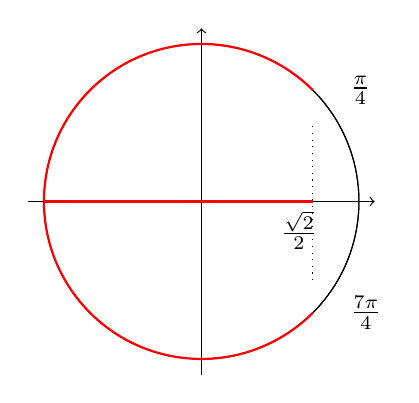
\begin{tikzpicture}[scale=2]
%Axes
\draw [->] (-1.1,0) -- (1.1,0);
\draw [->] (0,-1.1) -- (0,1.1);
%Cercle
\draw (0,0) circle (1);
%Intervalles axes
\draw [red,{-]}, thick] (-1,0) -- (0.707,0)  ;
%Traits
\draw [dotted] (0.707,-0.5) -- (0.707,0.5) ;
%Points
\draw (0.707,0) node[left, below] {$\ddp \frac{\sqrt{2}}{2} \quad$};
\draw (1,0) arc (0:-45:1) node[right] {$\quad \ddp \frac{7\pi}{4} $} ;
\draw (1,0) arc (0:45:1) node[right] {$\quad \ddp \frac{\pi}{4}$} ;
%Intervalles cercle
\draw [red, {-]}, thick] (-1,0) arc (180:45:1) ;
\draw [red, {-]}, thick] (-1,0) arc (-180:-45:1) ;
\end{tikzpicture}
\end{center}
\end{minipage}
Afin de donner les solutions dans $\lbrack 0,2\pi\lbrack$ et dans $\rbrack -\pi,\pi\rbrack$, on repr\'esente les solutions sur un cercle trigonom\'etrique en prenant $k=0,\ k=1$ et $k=2$. On obtient alors:
$$\fbox{$\mathcal{S}_{\lbrack 0,2\pi\lbrack}=\left\lbrack \ddp\frac{\pi}{12},\ddp\frac{7\pi}{12} \right\rbrack\cup\left\lbrack \ddp\frac{9\pi}{12},\ddp\frac{15\pi}{12} \right\rbrack\cup\left\lbrack \ddp\frac{17\pi}{12},\ddp\frac{23\pi}{12} \right\rbrack$}.$$
Et finalement :
$$\fbox{$ \mathcal{S}_{\rbrack -\pi,\pi\rbrack}=\left\rbrack -\pi,-\ddp\frac{9\pi}{12}  \right\rbrack\cup\left\lbrack -\ddp\frac{7\pi}{12},-\ddp\frac{\pi}{12} \right\rbrack\cup\left\lbrack \ddp\frac{\pi}{12},\ddp\frac{7\pi}{12} \right\rbrack\cup\left\lbrack \ddp\frac{9\pi}{12},\pi\right\rbrack$}.$$
%------------------------------
\item \textbf{R\'esolution de $\mathbf{ \tan{(x)}\leq 1 }$:}\\
\begin{minipage}[c]{0.45\textwidth}
\noindent La r\'esolution graphique sur le cercle trigonom\'etrique  donne :
$$\tan{(x)}\leq 1 \Leftrightarrow \exists k\in\Z,\ -\ddp\frac{\pi}{2}+k\pi < x\leq \ddp\frac{\pi}{4}+k\pi.$$
On obtient : \fbox{$ \mathcal{S}_{\R}= \ddp \mathop{\bigcup}\limits_{k\in \Z} \left] - \frac{\pi}{2} + k\pi, \frac{\pi}{4} + k \pi \right]$}.
\end{minipage}
\quad \begin{minipage}[c]{0.45\textwidth}
\begin{center}
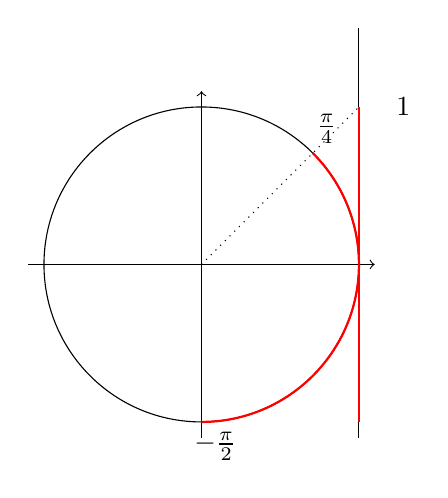
\begin{tikzpicture}[scale=2]
%Axes
\draw [->] (-1.1,0) -- (1.1,0);
\draw [->] (0,-1.1) -- (0,1.1);
\draw (1,-1.1) -- (1,1.5);
%Cercle
\draw (0,0) circle (1);
%Intervalles axes
\draw [red,{-]}, thick] (1,-1) -- (1,1);
%Traits
\draw [dotted] (0,0) -- (1,1) ;
%Points
\draw (1,1) node[right] {$\quad \ddp 1$};
\draw (1,0) arc (0:-90:1) node[below] {$\quad \ddp - \frac{\pi}{2} $} ;
\draw (1,0) arc (0:45:1) node[above] {$\quad \ddp \frac{\pi}{4}$} ;
%Intervalles cercle
\draw [red, {-]}, thick] (1,0) arc (0:45:1) ;
\draw [red, {-[}, thick] (1,0) arc (0:-90:1) ;
\end{tikzpicture}
\end{center}
\end{minipage}
Attention, les solutions pour la tangente sont d\'efinies modulo $\pi$, et non $2\pi$. Il y a donc deux intervalles solutions \`a tracer sur le cercle trigonom\'etrique.\\
\begin{minipage}[c]{0.45\textwidth}
On a donc : \fbox{$\mathcal{S}_{\lbrack 0,2\pi\lbrack}=\left\lbrack 0,\ddp\frac{\pi}{4}  \right\rbrack\cup \left\rbrack \ddp\frac{\pi}{2},\ddp\frac{5\pi}{4}  \right\rbrack\cup\left\rbrack \ddp\frac{3\pi}{2},2\pi  \right\lbrack$}.\\
Et finalement : \fbox{$ \mathcal{S}_{\rbrack -\pi,\pi\rbrack}=\left\rbrack -\pi,-\ddp\frac{3\pi}{4}  \right\rbrack\cup
\left\rbrack -\ddp\frac{\pi}{2},\ddp\frac{\pi}{4}  \right\rbrack\cup\left\rbrack \ddp\frac{\pi}{2},\pi  \right\rbrack
$}.
\end{minipage}
\quad \begin{minipage}[c]{0.45\textwidth}
\begin{center}
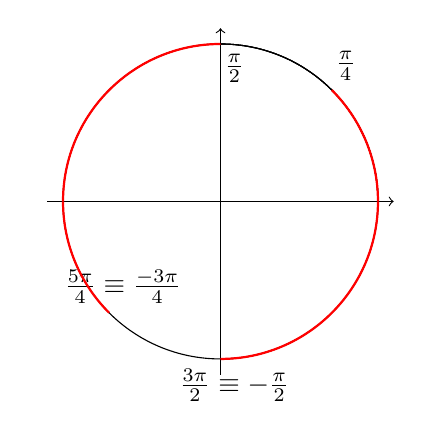
\begin{tikzpicture}[scale=2]
%Axes
\draw [->] (-1.1,0) -- (1.1,0);
\draw [->] (0,-1.1) -- (0,1.1);
%Cercle
\draw (0,0) circle (1);
%Points
\draw (1,0) arc (0:-90:1) node[below] {$\quad \ddp \frac{3\pi}{2} \equiv - \frac{\pi}{2}$} ;
\draw (1,0) arc (0:45:1) node[above] {$\quad \ddp \frac{\pi}{4}$} ;
\draw (1,0) arc (0:90:1) node[below] {$\quad \ddp  \frac{\pi}{2} $} ;
\draw (1,0) arc (0:225:1) node[above] {$\quad \ddp \frac{5\pi}{4} \equiv \frac{-3\pi}{4}$} ;
%Intervalles cercle
\draw [red, {-]}, thick] (1,0) arc (0:45:1) ;
\draw [red, {-[}, thick] (1,0) arc (0:-90:1) ;
\draw [red, {-[}, thick] (-1,0) arc (180:90:1) ;
\draw [red, {-]}, thick] (-1,0) arc (180:225:1) ;
\end{tikzpicture}
\end{center}
\end{minipage}
%------------------------------
\end{enumerate}
\end{correction}